\documentclass[twoside]{book}

% Packages required by doxygen
\usepackage{fixltx2e}
\usepackage{calc}
\usepackage{doxygen}
\usepackage[export]{adjustbox} % also loads graphicx
\usepackage{graphicx}
\usepackage[utf8]{inputenc}
\usepackage{makeidx}
\usepackage{multicol}
\usepackage{multirow}
\PassOptionsToPackage{warn}{textcomp}
\usepackage{textcomp}
\usepackage[nointegrals]{wasysym}
\usepackage[table]{xcolor}

% Font selection
\usepackage[T1]{fontenc}
\usepackage[scaled=.90]{helvet}
\usepackage{courier}
\usepackage{amssymb}
\usepackage{sectsty}
\renewcommand{\familydefault}{\sfdefault}
\allsectionsfont{%
  \fontseries{bc}\selectfont%
  \color{darkgray}%
}
\renewcommand{\DoxyLabelFont}{%
  \fontseries{bc}\selectfont%
  \color{darkgray}%
}
\newcommand{\+}{\discretionary{\mbox{\scriptsize$\hookleftarrow$}}{}{}}

% Page & text layout
\usepackage{geometry}
\geometry{%
  a4paper,%
  top=2.5cm,%
  bottom=2.5cm,%
  left=2.5cm,%
  right=2.5cm%
}
\tolerance=750
\hfuzz=15pt
\hbadness=750
\setlength{\emergencystretch}{15pt}
\setlength{\parindent}{0cm}
\setlength{\parskip}{0.2cm}
\makeatletter
\renewcommand{\paragraph}{%
  \@startsection{paragraph}{4}{0ex}{-1.0ex}{1.0ex}{%
    \normalfont\normalsize\bfseries\SS@parafont%
  }%
}
\renewcommand{\subparagraph}{%
  \@startsection{subparagraph}{5}{0ex}{-1.0ex}{1.0ex}{%
    \normalfont\normalsize\bfseries\SS@subparafont%
  }%
}
\makeatother

% Headers & footers
\usepackage{fancyhdr}
\pagestyle{fancyplain}
\fancyhead[LE]{\fancyplain{}{\bfseries\thepage}}
\fancyhead[CE]{\fancyplain{}{}}
\fancyhead[RE]{\fancyplain{}{\bfseries\leftmark}}
\fancyhead[LO]{\fancyplain{}{\bfseries\rightmark}}
\fancyhead[CO]{\fancyplain{}{}}
\fancyhead[RO]{\fancyplain{}{\bfseries\thepage}}
\fancyfoot[LE]{\fancyplain{}{}}
\fancyfoot[CE]{\fancyplain{}{}}
\fancyfoot[RE]{\fancyplain{}{\bfseries\scriptsize Generated on Wed Jan 21 2015 23\+:06\+:09 for Lib\+S\+D\+N\+B by Doxygen }}
\fancyfoot[LO]{\fancyplain{}{\bfseries\scriptsize Generated on Wed Jan 21 2015 23\+:06\+:09 for Lib\+S\+D\+N\+B by Doxygen }}
\fancyfoot[CO]{\fancyplain{}{}}
\fancyfoot[RO]{\fancyplain{}{}}
\renewcommand{\footrulewidth}{0.4pt}
\renewcommand{\chaptermark}[1]{%
  \markboth{#1}{}%
}
\renewcommand{\sectionmark}[1]{%
  \markright{\thesection\ #1}%
}

% Indices & bibliography
\usepackage{natbib}
\usepackage[titles]{tocloft}
\setcounter{tocdepth}{3}
\setcounter{secnumdepth}{5}
\makeindex

% Hyperlinks (required, but should be loaded last)
\usepackage{ifpdf}
\ifpdf
  \usepackage[pdftex,pagebackref=true]{hyperref}
\else
  \usepackage[ps2pdf,pagebackref=true]{hyperref}
\fi
\hypersetup{%
  colorlinks=true,%
  linkcolor=blue,%
  citecolor=blue,%
  unicode%
}

% Custom commands
\newcommand{\clearemptydoublepage}{%
  \newpage{\pagestyle{empty}\cleardoublepage}%
}


%===== C O N T E N T S =====

\begin{document}

% Titlepage & ToC
\hypersetup{pageanchor=false,
             bookmarks=true,
             bookmarksnumbered=true,
             pdfencoding=unicode
            }
\pagenumbering{roman}
\begin{titlepage}
\vspace*{7cm}
\begin{center}%
{\Large Lib\+S\+D\+N\+B \\[1ex]\large 0.\+0.\+0 }\\
\vspace*{1cm}
{\large Generated by Doxygen 1.8.9.1}\\
\vspace*{0.5cm}
{\small Wed Jan 21 2015 23:06:09}\\
\end{center}
\end{titlepage}
\clearemptydoublepage
\tableofcontents
\clearemptydoublepage
\pagenumbering{arabic}
\hypersetup{pageanchor=true}

%--- Begin generated contents ---
\chapter{Hierarchical Index}
\section{Class Hierarchy}
This inheritance list is sorted roughly, but not completely, alphabetically\+:\begin{DoxyCompactList}
\item \contentsline{section}{S\+D\+N\+B\+:\+:Gap\+Vector$<$ T $>$}{\pageref{classSDNB_1_1GapVector}}{}
\item iterator\begin{DoxyCompactList}
\item \contentsline{section}{S\+D\+N\+B\+:\+:Gap\+Vector$<$ T $>$\+:\+:iterator}{\pageref{classSDNB_1_1GapVector_1_1iterator}}{}
\end{DoxyCompactList}
\end{DoxyCompactList}

\chapter{Class Index}
\section{Class List}
Here are the classes, structs, unions and interfaces with brief descriptions\+:\begin{DoxyCompactList}
\item\contentsline{section}{\hyperlink{classSDNB_1_1GapVector}{S\+D\+N\+B\+::\+Gap\+Vector$<$ T $>$} \\*\hyperlink{classSDNB_1_1GapVector}{Gap\+Vector} class }{\pageref{classSDNB_1_1GapVector}}{}
\item\contentsline{section}{\hyperlink{classSDNB_1_1GapVector_1_1iterator}{S\+D\+N\+B\+::\+Gap\+Vector$<$ T $>$\+::iterator} }{\pageref{classSDNB_1_1GapVector_1_1iterator}}{}
\end{DoxyCompactList}

\chapter{Class Documentation}
\hypertarget{classSDNB_1_1GapVector}{}\section{S\+D\+N\+B\+:\+:Gap\+Vector$<$ T $>$ Class Template Reference}
\label{classSDNB_1_1GapVector}\index{S\+D\+N\+B\+::\+Gap\+Vector$<$ T $>$@{S\+D\+N\+B\+::\+Gap\+Vector$<$ T $>$}}


\hyperlink{classSDNB_1_1GapVector}{Gap\+Vector} class.  




{\ttfamily \#include $<$gap\+\_\+vector.\+hh$>$}

\subsection*{Classes}
\begin{DoxyCompactItemize}
\item 
class \hyperlink{classSDNB_1_1GapVector_1_1iterator}{iterator}
\end{DoxyCompactItemize}
\subsection*{Public Types}
\begin{DoxyCompactItemize}
\item 
\hypertarget{classSDNB_1_1GapVector_a5f7b534c044fec7f25fa430c88fd167e}{}typedef const \hyperlink{classSDNB_1_1GapVector_1_1iterator}{iterator} {\bfseries const\+\_\+iterator}\label{classSDNB_1_1GapVector_a5f7b534c044fec7f25fa430c88fd167e}

\item 
\hypertarget{classSDNB_1_1GapVector_aa2476e7a8104ca8d5b61f7873b76a18e}{}typedef std\+::reverse\+\_\+iterator$<$ \hyperlink{classSDNB_1_1GapVector_1_1iterator}{iterator} $>$ {\bfseries reverse\+\_\+iterator}\label{classSDNB_1_1GapVector_aa2476e7a8104ca8d5b61f7873b76a18e}

\item 
\hypertarget{classSDNB_1_1GapVector_a37c5f4d092df95a05852a9d3014e9bf4}{}typedef std\+::reverse\+\_\+iterator$<$ \hyperlink{classSDNB_1_1GapVector_1_1iterator}{const\+\_\+iterator} $>$ {\bfseries const\+\_\+reverse\+\_\+iterator}\label{classSDNB_1_1GapVector_a37c5f4d092df95a05852a9d3014e9bf4}

\end{DoxyCompactItemize}
\subsection*{Public Member Functions}
\begin{DoxyCompactItemize}
\item 
\hypertarget{classSDNB_1_1GapVector_ae2017ba1405b81d73fa8db9a53fd475d}{}{\bfseries Gap\+Vector} (size\+\_\+t size=128)\label{classSDNB_1_1GapVector_ae2017ba1405b81d73fa8db9a53fd475d}

\item 
\hypertarget{classSDNB_1_1GapVector_adc12d325e3d9473e959ad57031a413ff}{}{\bfseries Gap\+Vector} (const \hyperlink{classSDNB_1_1GapVector}{Gap\+Vector} \&arg)\label{classSDNB_1_1GapVector_adc12d325e3d9473e959ad57031a413ff}

\item 
\hypertarget{classSDNB_1_1GapVector_a811a405824301979b0a2cb957834bb39}{}\hyperlink{classSDNB_1_1GapVector}{Gap\+Vector} \& {\bfseries operator=} (\hyperlink{classSDNB_1_1GapVector}{Gap\+Vector} arg)\label{classSDNB_1_1GapVector_a811a405824301979b0a2cb957834bb39}

\item 
\hypertarget{classSDNB_1_1GapVector_a7e3163451ad54ce89a80837b3bdc622d}{}\hyperlink{classSDNB_1_1GapVector}{Gap\+Vector} \& {\bfseries operator=} (const \hyperlink{classSDNB_1_1GapVector}{Gap\+Vector} \&arg)\label{classSDNB_1_1GapVector_a7e3163451ad54ce89a80837b3bdc622d}

\item 
\hypertarget{classSDNB_1_1GapVector_aef1d8380623e93dad6f49ec3dcf6ddfa}{}T \& {\bfseries operator\mbox{[}$\,$\mbox{]}} (size\+\_\+t index)\label{classSDNB_1_1GapVector_aef1d8380623e93dad6f49ec3dcf6ddfa}

\item 
\hypertarget{classSDNB_1_1GapVector_aaf3510f16fa61ef5db2e8b9bb443c218}{}const T \& {\bfseries operator\mbox{[}$\,$\mbox{]}} (size\+\_\+t index) const \label{classSDNB_1_1GapVector_aaf3510f16fa61ef5db2e8b9bb443c218}

\item 
\hypertarget{classSDNB_1_1GapVector_a45a4d64f4094416c853e906e89992a2d}{}{\footnotesize template$<$class iter $>$ }\\void {\bfseries insert} (iter first, iter last)\label{classSDNB_1_1GapVector_a45a4d64f4094416c853e906e89992a2d}

\item 
\hypertarget{classSDNB_1_1GapVector_a5165204380dc464053e3ee326e49b81f}{}int {\bfseries remove} (int length)\label{classSDNB_1_1GapVector_a5165204380dc464053e3ee326e49b81f}

\item 
\hypertarget{classSDNB_1_1GapVector_aac2ca857e4e2edc83734fe4314c21740}{}int {\bfseries move\+Gap} (int distance)\label{classSDNB_1_1GapVector_aac2ca857e4e2edc83734fe4314c21740}

\item 
\hypertarget{classSDNB_1_1GapVector_a3e9629fd65899c8861d9b8a3ee80e838}{}\hyperlink{classSDNB_1_1GapVector_1_1iterator}{iterator} {\bfseries begin} (void)\label{classSDNB_1_1GapVector_a3e9629fd65899c8861d9b8a3ee80e838}

\item 
\hypertarget{classSDNB_1_1GapVector_ad0dcea81f55ae8970e65e4778da37abb}{}reverse\+\_\+iterator {\bfseries rbegin} (void)\label{classSDNB_1_1GapVector_ad0dcea81f55ae8970e65e4778da37abb}

\item 
\hypertarget{classSDNB_1_1GapVector_a124b2683624fe7ad8a76d3b9b6027b7d}{}\hyperlink{classSDNB_1_1GapVector_1_1iterator}{iterator} {\bfseries end} (void)\label{classSDNB_1_1GapVector_a124b2683624fe7ad8a76d3b9b6027b7d}

\item 
\hypertarget{classSDNB_1_1GapVector_aba393fa2eb30e00623183c986c8fb0e9}{}reverse\+\_\+iterator {\bfseries rend} (void)\label{classSDNB_1_1GapVector_aba393fa2eb30e00623183c986c8fb0e9}

\item 
\hypertarget{classSDNB_1_1GapVector_a556e1db779dbe48ade40bd2040116b9c}{}\hyperlink{classSDNB_1_1GapVector_1_1iterator}{iterator} {\bfseries gap} (void)\label{classSDNB_1_1GapVector_a556e1db779dbe48ade40bd2040116b9c}

\item 
\hypertarget{classSDNB_1_1GapVector_a6cd2a4e619a689aac9a0132e7110de2b}{}reverse\+\_\+iterator {\bfseries rgap} (void)\label{classSDNB_1_1GapVector_a6cd2a4e619a689aac9a0132e7110de2b}

\end{DoxyCompactItemize}
\subsection*{Public Attributes}
\begin{DoxyCompactItemize}
\item 
\hypertarget{classSDNB_1_1GapVector_a0749dee549dbbf9dc3819ff74415ee82}{}size\+\_\+t {\bfseries size}\label{classSDNB_1_1GapVector_a0749dee549dbbf9dc3819ff74415ee82}

\end{DoxyCompactItemize}
\subsection*{Protected Attributes}
\begin{DoxyCompactItemize}
\item 
\hypertarget{classSDNB_1_1GapVector_a279ce160457349d958452816dfa6d9cf}{}const size\+\_\+t {\bfseries \+\_\+default\+Gap\+Size}\label{classSDNB_1_1GapVector_a279ce160457349d958452816dfa6d9cf}

\end{DoxyCompactItemize}
\subsection*{Friends}
\begin{DoxyCompactItemize}
\item 
\hypertarget{classSDNB_1_1GapVector_a67171474c4da6cc8efe0c7fafefd2b2d}{}class {\bfseries iterator}\label{classSDNB_1_1GapVector_a67171474c4da6cc8efe0c7fafefd2b2d}

\end{DoxyCompactItemize}


\subsection{Detailed Description}
\subsubsection*{template$<$class T$>$class S\+D\+N\+B\+::\+Gap\+Vector$<$ T $>$}

\hyperlink{classSDNB_1_1GapVector}{Gap\+Vector} class. 

The \hyperlink{classSDNB_1_1GapVector}{Gap\+Vector} Class is a templatized version of a gap buffer data structure. The class conforms to C++ S\+T\+L style and implements a random access iterator. 

The documentation for this class was generated from the following file\+:\begin{DoxyCompactItemize}
\item 
src/sdnb/headers/gap\+\_\+vector.\+hh\end{DoxyCompactItemize}

\hypertarget{classSDNB_1_1GapVector_1_1iterator}{}\section{S\+D\+N\+B\+:\+:Gap\+Vector$<$ T $>$\+:\+:iterator Class Reference}
\label{classSDNB_1_1GapVector_1_1iterator}\index{S\+D\+N\+B\+::\+Gap\+Vector$<$ T $>$\+::iterator@{S\+D\+N\+B\+::\+Gap\+Vector$<$ T $>$\+::iterator}}
Inheritance diagram for S\+D\+N\+B\+:\+:Gap\+Vector$<$ T $>$\+:\+:iterator\+:\begin{figure}[H]
\begin{center}
\leavevmode
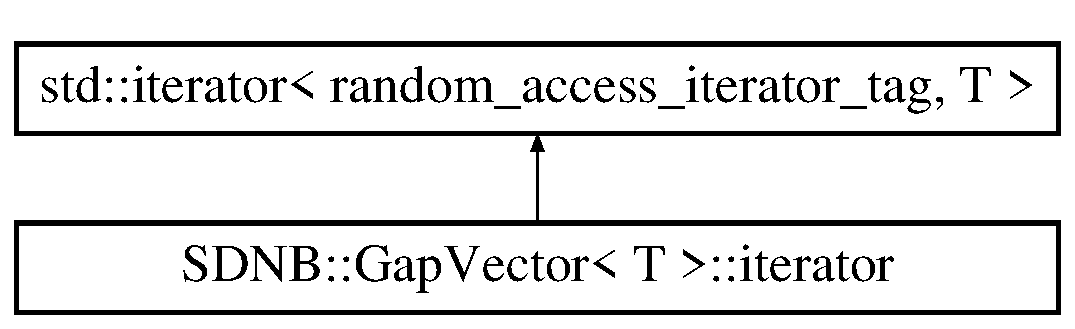
\includegraphics[height=2.000000cm]{classSDNB_1_1GapVector_1_1iterator}
\end{center}
\end{figure}
\subsection*{Public Member Functions}
\begin{DoxyCompactItemize}
\item 
\hypertarget{classSDNB_1_1GapVector_1_1iterator_a5a38809ed11832257cf5bfb8a5dbee98}{}{\bfseries iterator} (\hyperlink{classSDNB_1_1GapVector}{Gap\+Vector}$<$ T $>$ $\ast$arg)\label{classSDNB_1_1GapVector_1_1iterator_a5a38809ed11832257cf5bfb8a5dbee98}

\item 
\hypertarget{classSDNB_1_1GapVector_1_1iterator_ad302ecb41a494c59a6733e4733d51c75}{}\hyperlink{classSDNB_1_1GapVector_1_1iterator}{iterator} \& {\bfseries operator=} (\hyperlink{classSDNB_1_1GapVector_1_1iterator}{iterator} arg)\label{classSDNB_1_1GapVector_1_1iterator_ad302ecb41a494c59a6733e4733d51c75}

\item 
\hypertarget{classSDNB_1_1GapVector_1_1iterator_ad2905b4855e9b2ce5866f6d21c067167}{}\hyperlink{classSDNB_1_1GapVector_1_1iterator}{iterator} \& {\bfseries operator++} (void)\label{classSDNB_1_1GapVector_1_1iterator_ad2905b4855e9b2ce5866f6d21c067167}

\item 
\hypertarget{classSDNB_1_1GapVector_1_1iterator_a6586094b0103c205fdca97930a19d57a}{}\hyperlink{classSDNB_1_1GapVector_1_1iterator}{iterator} {\bfseries operator++} (int)\label{classSDNB_1_1GapVector_1_1iterator_a6586094b0103c205fdca97930a19d57a}

\item 
\hypertarget{classSDNB_1_1GapVector_1_1iterator_a713212b2c288556180bf815bd88f33cc}{}\hyperlink{classSDNB_1_1GapVector_1_1iterator}{iterator} \& {\bfseries operator+=} (int offset)\label{classSDNB_1_1GapVector_1_1iterator_a713212b2c288556180bf815bd88f33cc}

\item 
\hypertarget{classSDNB_1_1GapVector_1_1iterator_a7f66471133e7c1093aed29f28149c7fb}{}\hyperlink{classSDNB_1_1GapVector_1_1iterator}{iterator} \& {\bfseries operator-\/-\/} (void)\label{classSDNB_1_1GapVector_1_1iterator_a7f66471133e7c1093aed29f28149c7fb}

\item 
\hypertarget{classSDNB_1_1GapVector_1_1iterator_ad34cbcc1adfa981799c40e9f6a8eefd0}{}\hyperlink{classSDNB_1_1GapVector_1_1iterator}{iterator} {\bfseries operator-\/-\/} (int)\label{classSDNB_1_1GapVector_1_1iterator_ad34cbcc1adfa981799c40e9f6a8eefd0}

\item 
\hypertarget{classSDNB_1_1GapVector_1_1iterator_a42c07395410700685743bd2952707ff4}{}\hyperlink{classSDNB_1_1GapVector_1_1iterator}{iterator} \& {\bfseries operator-\/=} (int offset)\label{classSDNB_1_1GapVector_1_1iterator_a42c07395410700685743bd2952707ff4}

\item 
\hypertarget{classSDNB_1_1GapVector_1_1iterator_a09bc6e725d8260f1560ae78cd67c16f0}{}T \& {\bfseries operator$\ast$} (void)\label{classSDNB_1_1GapVector_1_1iterator_a09bc6e725d8260f1560ae78cd67c16f0}

\item 
\hypertarget{classSDNB_1_1GapVector_1_1iterator_a12e6dac2e3b6eae755e19ba52a7e6e8c}{}bool {\bfseries operator==} (const \hyperlink{classSDNB_1_1GapVector_1_1iterator}{iterator} \&rhs)\label{classSDNB_1_1GapVector_1_1iterator_a12e6dac2e3b6eae755e19ba52a7e6e8c}

\item 
\hypertarget{classSDNB_1_1GapVector_1_1iterator_a92c68f0809e36fbed1e96a45d22758ed}{}bool {\bfseries operator!=} (const \hyperlink{classSDNB_1_1GapVector_1_1iterator}{iterator} \&rhs)\label{classSDNB_1_1GapVector_1_1iterator_a92c68f0809e36fbed1e96a45d22758ed}

\item 
\hypertarget{classSDNB_1_1GapVector_1_1iterator_aa1bc85efd2b77ba6977b4c8740310f6b}{}bool {\bfseries operator$<$} (const \hyperlink{classSDNB_1_1GapVector_1_1iterator}{iterator} \&rhs)\label{classSDNB_1_1GapVector_1_1iterator_aa1bc85efd2b77ba6977b4c8740310f6b}

\item 
\hypertarget{classSDNB_1_1GapVector_1_1iterator_a2be7ca3bfd966f252e3ade1c17298e3b}{}bool {\bfseries operator$>$} (const \hyperlink{classSDNB_1_1GapVector_1_1iterator}{iterator} \&rhs)\label{classSDNB_1_1GapVector_1_1iterator_a2be7ca3bfd966f252e3ade1c17298e3b}

\item 
\hypertarget{classSDNB_1_1GapVector_1_1iterator_a43692447cc21df3af5f39c0f8603e0c8}{}bool {\bfseries operator$<$=} (const \hyperlink{classSDNB_1_1GapVector_1_1iterator}{iterator} \&rhs)\label{classSDNB_1_1GapVector_1_1iterator_a43692447cc21df3af5f39c0f8603e0c8}

\item 
\hypertarget{classSDNB_1_1GapVector_1_1iterator_a56ee00a5aba2dd4fe8d497303a4aad5b}{}bool {\bfseries operator$>$=} (const \hyperlink{classSDNB_1_1GapVector_1_1iterator}{iterator} \&rhs)\label{classSDNB_1_1GapVector_1_1iterator_a56ee00a5aba2dd4fe8d497303a4aad5b}

\item 
\hypertarget{classSDNB_1_1GapVector_1_1iterator_a0794000c4e8173ba998ac69ec8441b31}{}T \& {\bfseries operator\mbox{[}$\,$\mbox{]}} (size\+\_\+t offset)\label{classSDNB_1_1GapVector_1_1iterator_a0794000c4e8173ba998ac69ec8441b31}

\item 
\hypertarget{classSDNB_1_1GapVector_1_1iterator_a0b5ad4d1b4c4050a6b221c938d8a360c}{}const T \& {\bfseries operator\mbox{[}$\,$\mbox{]}} (size\+\_\+t offset) const \label{classSDNB_1_1GapVector_1_1iterator_a0b5ad4d1b4c4050a6b221c938d8a360c}

\end{DoxyCompactItemize}
\subsection*{Friends}
\begin{DoxyCompactItemize}
\item 
\hypertarget{classSDNB_1_1GapVector_1_1iterator_ad276f1b756293ba5e93da0a53bb02996}{}\hyperlink{classSDNB_1_1GapVector_1_1iterator}{iterator} {\bfseries operator+} (\hyperlink{classSDNB_1_1GapVector_1_1iterator}{iterator} it, int offset)\label{classSDNB_1_1GapVector_1_1iterator_ad276f1b756293ba5e93da0a53bb02996}

\item 
\hypertarget{classSDNB_1_1GapVector_1_1iterator_ab3bcd660aaf8ec01c51e2f65f011c7d9}{}\hyperlink{classSDNB_1_1GapVector_1_1iterator}{iterator} {\bfseries operator+} (int offset, const \hyperlink{classSDNB_1_1GapVector_1_1iterator}{iterator} \&it)\label{classSDNB_1_1GapVector_1_1iterator_ab3bcd660aaf8ec01c51e2f65f011c7d9}

\item 
\hypertarget{classSDNB_1_1GapVector_1_1iterator_aa5112bbfcc346bf466075266f6862228}{}\hyperlink{classSDNB_1_1GapVector_1_1iterator}{iterator} {\bfseries operator-\/} (\hyperlink{classSDNB_1_1GapVector_1_1iterator}{iterator} it, int offset)\label{classSDNB_1_1GapVector_1_1iterator_aa5112bbfcc346bf466075266f6862228}

\item 
\hypertarget{classSDNB_1_1GapVector_1_1iterator_a8190f6ba087cab1c57a8f87d9403f6ae}{}\hyperlink{classSDNB_1_1GapVector_1_1iterator}{iterator} {\bfseries operator-\/} (int offset, const \hyperlink{classSDNB_1_1GapVector_1_1iterator}{iterator} \&it)\label{classSDNB_1_1GapVector_1_1iterator_a8190f6ba087cab1c57a8f87d9403f6ae}

\item 
\hypertarget{classSDNB_1_1GapVector_1_1iterator_a41d99fcef815c2090e57789a8ac73486}{}int {\bfseries operator-\/} (\hyperlink{classSDNB_1_1GapVector_1_1iterator}{iterator} lhs, const \hyperlink{classSDNB_1_1GapVector_1_1iterator}{iterator} \&rhs)\label{classSDNB_1_1GapVector_1_1iterator_a41d99fcef815c2090e57789a8ac73486}

\end{DoxyCompactItemize}


The documentation for this class was generated from the following file\+:\begin{DoxyCompactItemize}
\item 
src/sdnb/headers/gap\+\_\+vector.\+hh\end{DoxyCompactItemize}

%--- End generated contents ---

% Index
\backmatter
\newpage
\phantomsection
\clearemptydoublepage
\addcontentsline{toc}{chapter}{Index}
\printindex

\end{document}
